\section{Appendix}

\subsection{Implementation Details}
% \Cref{tab:hyperparameters} summarizes the hyperparameter configurations for the D-FINE models, including D-FINE-X, D-FINE-L, D-FINE-M, and D-FINE-S. All models utilize HGNetV2 backbones (versions B0 to B5) and the AdamW optimizer. The embedding dimensions are set to 384 for D-FINE-X and 256 for the other variants, while feedforward dimensions are 2048 for D-FINE-X and 1024 for D-FINE-L, D-FINE-M, and D-FINE-S. The GELAN hidden dimensions and depths are tailored per model, with D-FINE-X having the highest (192 and 3) and D-FINE-S the lowest (64 and 1). During training, each model employs one encoder layer and one decoder layer, whereas evaluation uses up to six decoder layers for D-FINE-X and D-FINE-L, and four for D-FINE-M and D-FINE-S. All models maintain 300 queries, a bin number of 32, and consistent sampling points (S: 3, M: 6, L: 3) with a temperature of 5. The base learning rate is set to 2.5e-4, with a slightly reduced learning rate for the backbone in D-FINE-L, D-FINE-M, and D-FINE-S. Weight decay is uniformly applied at 1.25e-4, and loss component weights are fine-tuned for each model. An EMA decay of 0.9999 is used across all models. Training schedules vary, with D-FINE-X and D-FINE-L trained for 72 epochs (including 2 without augmentation) and D-FINE-M and D-FINE-S for 120 epochs (including 3 without augmentation). These carefully selected hyperparameters ensure optimal performance and efficiency for each D-FINE model variant.
\subsubsection{Hyperparameter Configurations}
\label{sec:hyper}
\Cref{tab:hyperparameters} summarizes the hyperparameter configurations for the D-FINE models. All variants use HGNetV2 backbones pretrained on ImageNet~\citep{cui2021selfsupervisionsimpleeffectivenetwork, russakovsky2015imagenet} and the AdamW optimizer. D-FINE-X is set with an embedding dimension of 384 and a feedforward dimension of 2048, while the other models use 256 and 1024, respectively. The D-FINE-X and D-FINE-L have 6 decoder layers, while D-FINE-M and D-FINE-S have 4 and 3 decoder layers. The GELAN module progressively reduces hidden dimension and depth from D-FINE-X with 192 dimensions and 3 layers to D-FINE-S with 64 dimensions and 1 layer. The base learning rate and weight decay for D-FINE-X and D-FINE-L are $2.5 \times 10^{-4}$ and $1.25 \times 10^{-4}$, respectively, while D-FINE-M and D-FINE-S use $2 \times 10^{-4}$ and $1 \times 10^{-4}$. Smaller models also have higher backbone learning rates than larger models. The total batch size is 32 across all variants. Training schedules include 72 epochs with advanced augmentation (\texttt{RandomPhotometricDistort, RandomZoomOut, RandomIoUCrop}, and \texttt{RMultiScaleInput}) followed by 2 epochs without advanced augmentation for D-FINE-X and D-FINE-L, and 120 epochs with advanced augmentation followed by 4 epochs without advanced augmentation for D-FINE-M and D-FINE-S (RT-DETRv2 Training Strategy~\citep{lv2024rtdetrv2} in \Cref{tab:model_modifications}). The number of pretraining epochs is 21 for D-FINE-X and D-FINE-L models, while for D-FINE-M and D-FINE-S models, it ranges from 28 to 29 epochs.

\begin{table}[ht]
\caption{Hyperparameter configurations for different D-FINE models.}
\begin{center}
\begin{adjustbox}{width=\columnwidth}
\begin{tabular}{l|cccc}
\multicolumn{5}{l}{}\\
\toprule
\textbf{Setting} & \textbf{D-FINE-X} & \textbf{D-FINE-L} & \textbf{D-FINE-M} & \textbf{D-FINE-S} \\
\midrule
Backbone Name & HGNetv2-B5 & HGNetv2-B4 & HGNetv2-B2 & HGNetv2-B0 \\
Optimizer & AdamW & AdamW & AdamW & AdamW \\
Embedding Dimension & 384 & 256 & 256 & 256 \\
Feedforward Dimension & 2048 & 1024 & 1024 & 1024 \\
GELAN Hidden Dimension & 192 & 128 & 128 & 64 \\
GELAN Depth & 3 & 3 & 2 & 1 \\
Decoder Layers & 6 & 6 & 4 & 3 \\
Queries & 300 & 300 & 300 & 300 \\
$a$,\ $c$ in $W(n)$ & 0.5,\ 0.125 & 0.5,\ 0.25 & 0.5,\ 0.25 & 0.5,\ 0.25 \\
Bin Number $N$ & 32 & 32 & 32 & 32 \\
Sampling Point Number & (S: 3, M: 6, L: 3) & (S: 3, M: 6, L: 3) & (S: 3, M: 6, L: 3) & (S: 3, M: 6, L: 3) \\
Temporature $T$ & 5 & 5 & 5 & 5 \\
Base LR & 2.5e-4 & 2.5e-4 & 2e-4 & 2e-4 \\
Backbone LR & 2.5e-6 & 1.25e-5 & 2e-5 & 1e-4 \\
Weight Decay & 1.25e-4 & 1.25e-4 & 1e-4 & 1e-4 \\
Weight of $\mathcal{L}_{\text{VFL}}$ & 1 & 1 & 1 & 1 \\
Weight of $\mathcal{L}_{\text{BBox}}$ & 5 & 5 & 5 & 5 \\
Weight of $\mathcal{L}_{\text{GIOU}}$ & 2 & 2 & 2 & 2 \\
Weight of $\mathcal{L}_{\text{FGL}}$ & 0.15 & 0.15 & 0.15 & 0.15 \\
Weight of $\mathcal{L}_{\text{DDF}}$ & 1.5 & 1.5 & 1.5 & 1.5 \\
Total Batch Size & 32 & 32 & 32 & 32 \\
EMA Decay & 0.9999 & 0.9999 & 0.9999 & 0.9999 \\
Epochs (w/ + w/o Adv. Aug.) & 72 + 2 & 72 + 2 & 120 + 4 & 120 + 4 \\
Epochs (Pretrain + Finetune) & 21 + 31 & 21 + 32 & 29 + 49 & 28 + 58 \\
\bottomrule
\end{tabular}
\end{adjustbox}
\end{center}
\label{tab:hyperparameters}
\end{table}


\subsubsection{Datasets Settings}
For pretraining, following the approach in~\citep{chen2022groupdetrv2strong, zhang2022dino, chen2024lw}, we combine the images from the Objects365~\citep{shao2019objects365} train set with the validate set, excluding the first 5k images. To further improve training efficiency, we resize all images with resolutions exceeding $640\times640$ down to $640\times640$ beforehand. We use the standard COCO2017~\citep{lin2014microsoft} data splitting policy, training on COCO \texttt{train2017}, and evaluating on COCO \texttt{val2017}.

% \subsubsection{YOLOv10 Pretraining}
% Following the pretraining protocol of YOLOv8~\citep{yolov8}, YOLOv10 was pretrained on the Objects365 dataset~\citep{shao2019objects365} for 300 epochs. 

\subsection{Visualization of D-FINE Predictions}
% \Cref{fig:hard} illustrates the detection predictions of D-FINE in complex scenarios and challenging conditions on the COCO \texttt{val2017} dataset. D-FINE exhibits robust detection capabilities under challenging conditions, such as severe occlusion, motion blur, rotation settings, and objects with varying orientations. These examples highlight the superior ability of D-FINE to handle diverse and difficult detection tasks, demonstrating its effectiveness in real-world applications.
\Cref{fig:hard} demonstrates the robustness of the D-FINE-X model, visualizing its predictions in various challenging scenarios. These include occlusion, low-light conditions, motion blur, depth of field effects, rotation, and densely populated scenes with numerous objects in close proximity. Despite these difficulties, the model accurately identifies and localizes objects, such as animals, vehicles, and people. This visualization highlights the model's ability to handle complex real-world conditions while maintaining robust detection performance.
\begin{figure}[ht]
    \centering
        \centering
        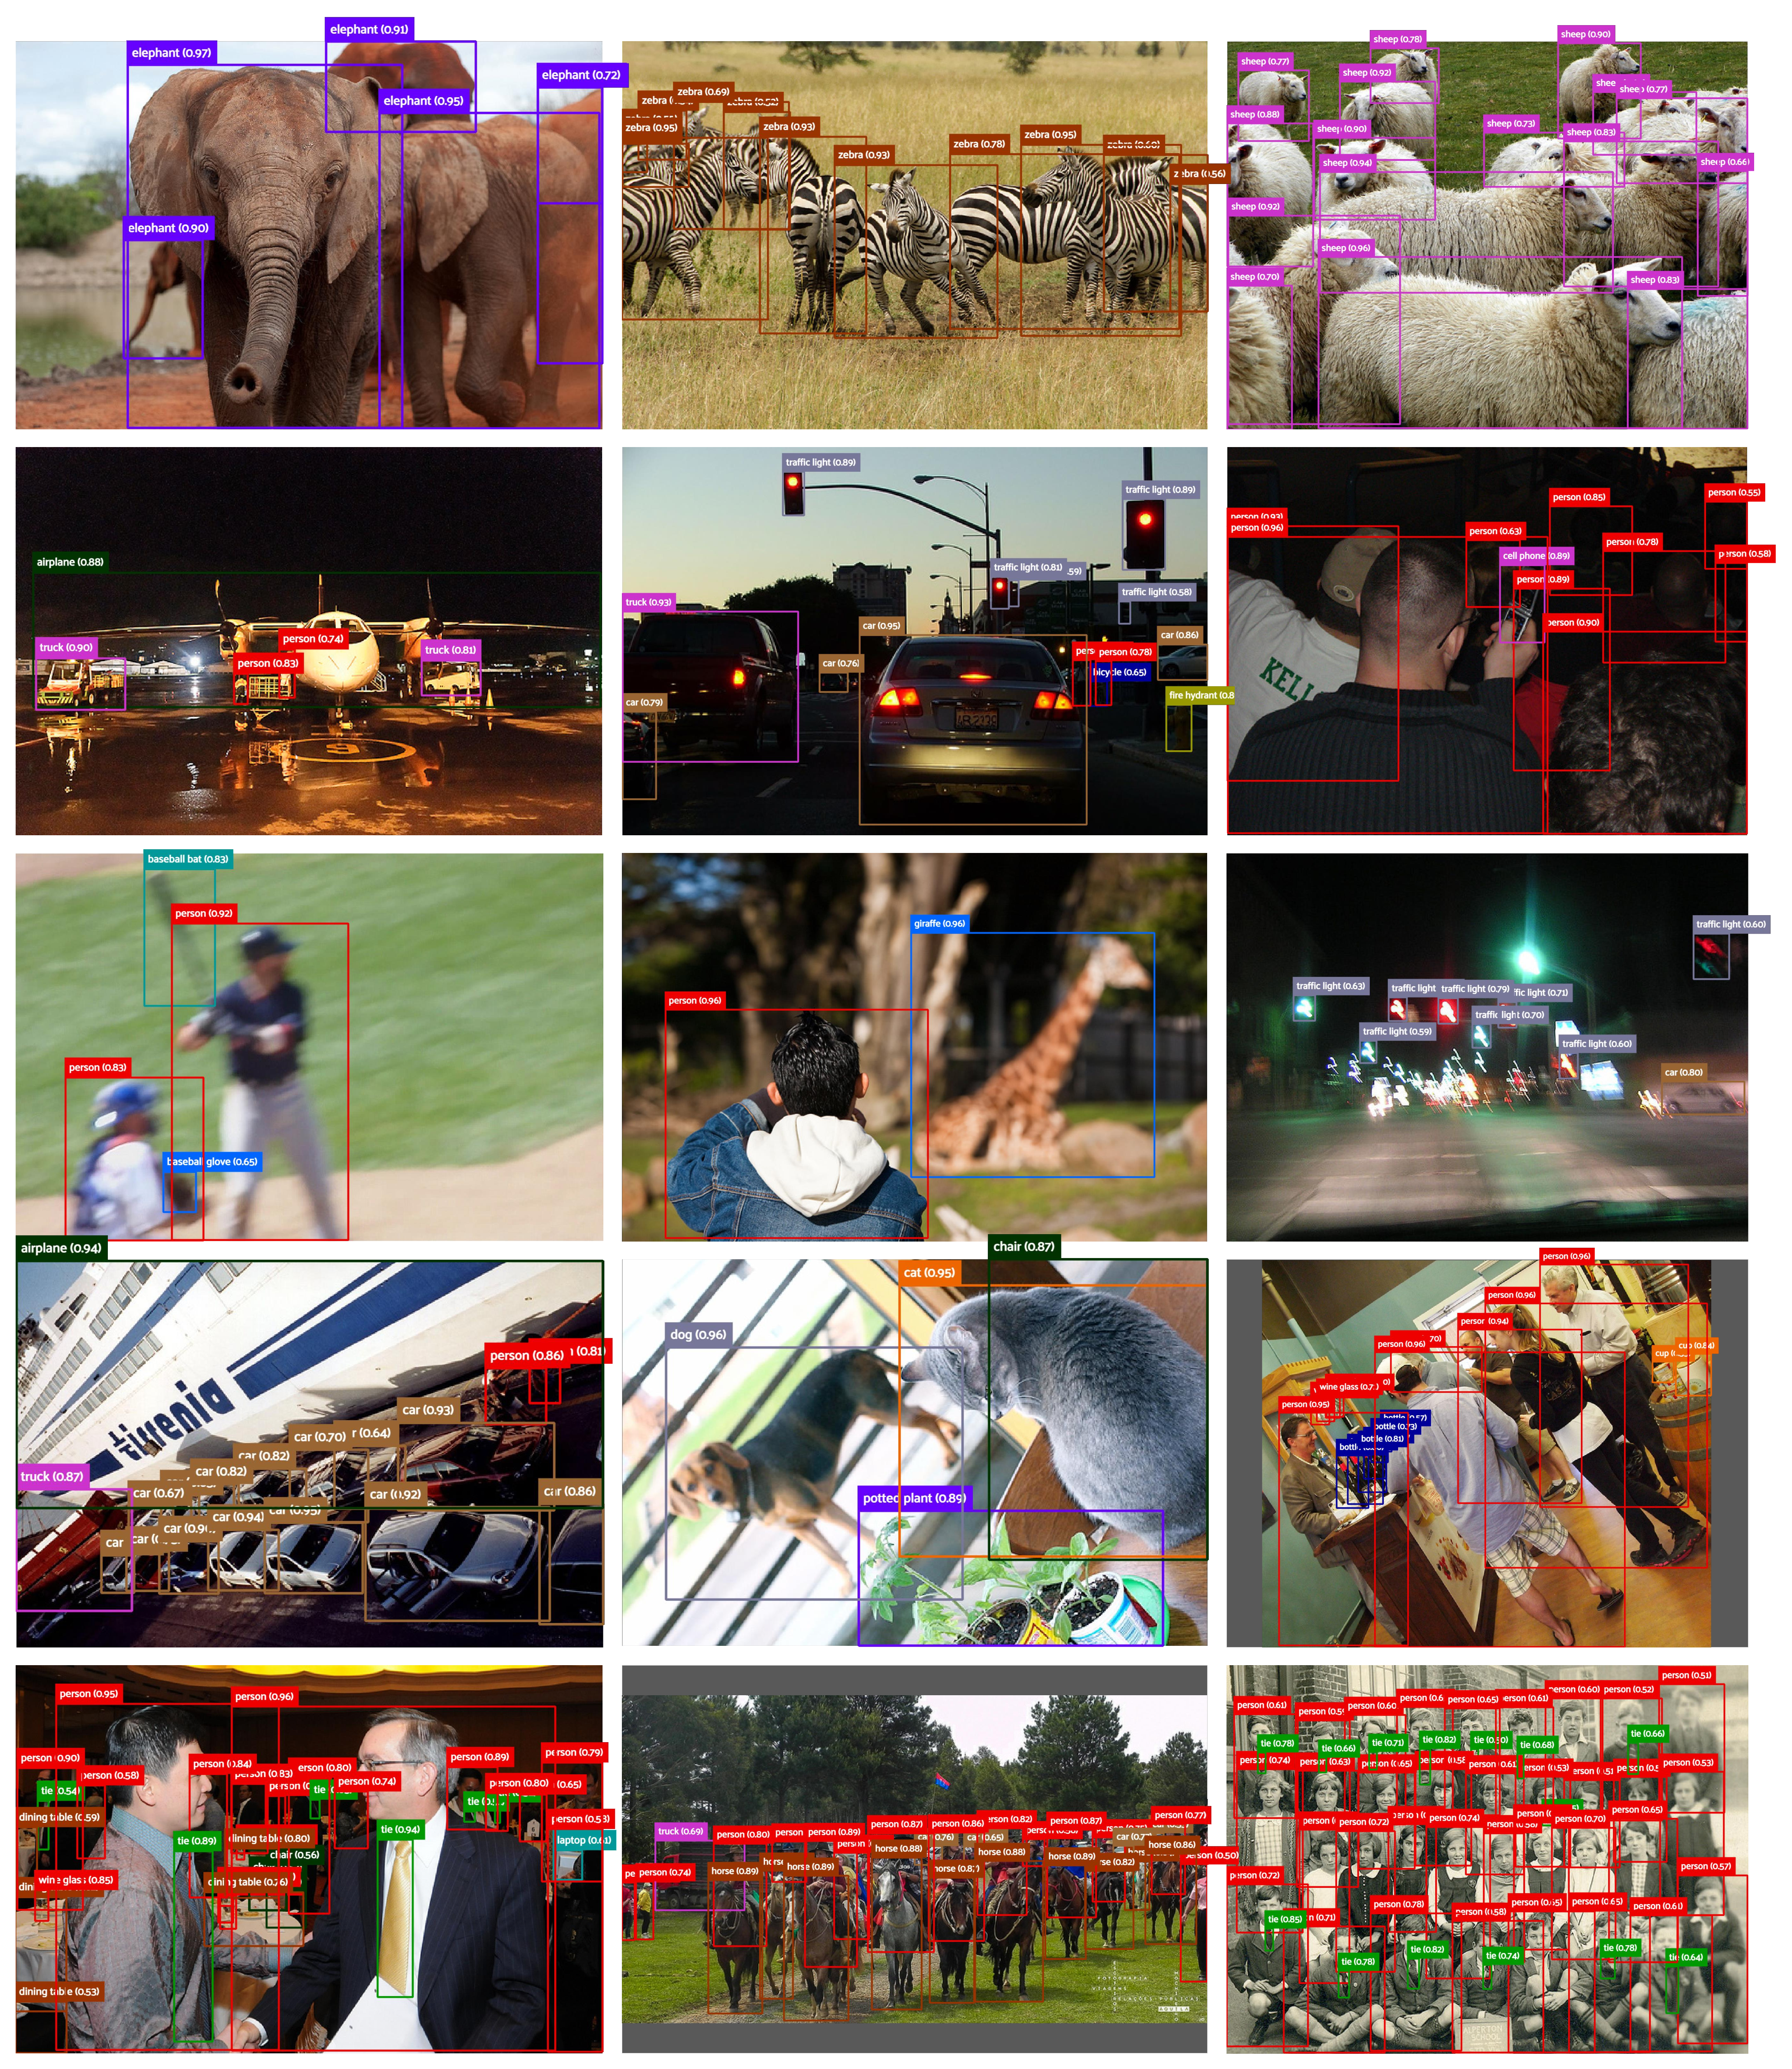
\includegraphics[width=\textwidth]{fig/hard_case.pdf}
        \caption{Visualization of D-FINE-X (without pre-training on Objects365) predictions under challenging conditions, including occlusion, low light, motion blur, depth of field effects, rotation, and densely populated scenes (confidence threshold=0.5).}

    \label{fig:hard}
\end{figure}


\subsection{Comparison with Lighter Detectors}
\Cref{tab:model_of_SM} presents a comprehensive comparison of D-FINE models with various lightweight real-time object detectors in the S and M model sizes on the COCO \texttt{val2017}. D-FINE-S achieves an impressive AP of 48.5\%, surpassing other lightweight models such as Gold-YOLO-S (46.4\%) and RT-DETRv2-S (48.1\%), while maintaining a low latency of 3.49 ms with only 10.2M parameters and 25.2 GFLOPs. Pretraining on Objects365 further boosts D-FINE-S to 50.7\%, marking an improvement of +2.2\%. Similarly, D-FINE-M attains an AP of 52.3\% with 19.2M parameters and 56.6 GFLOPs at 5.62 ms, outperforming YOLOv10-M (51.1\%) and RT-DETRv2-M (49.9\%). Pretraining on Objects365 consistently enhances D-FINE-M, yielding a +2.8\% gain. These results demonstrate that D-FINE models strike an excellent balance between accuracy and efficiency, consistently surpassing other state-of-the-art lightweight detectors while preserving real-time performance.

\begin{table}[ht]
    \caption{Performance comparison of S and M sized real-time object detectors on COCO \texttt{val2017}.}
    \begin{center}
    \begin{adjustbox}{width=\columnwidth}
    \begin{tabular}{l | ccc | ccc ccc}
    \toprule
    \hline
        Model & \#Params. & GFLOPs & Latency (ms) & AP$^{val}$ & AP$^{val}_{50}$ & AP$^{val}_{75}$ & AP$^{val}_S$ & AP$^{val}_M$ & AP$^{val}_L$ \\
    \midrule
    \hline
    \rowcolor{f2ecde}
    \multicolumn{10}{l}{\emph{Non-end-to-end Real-time Object Detectors}} \\
    YOLOv6-S & 7M & 17 & 3.62 & 45.0 & 61.8 & 48.9 & 24.3 & 50.2 & 62.7 \\
    YOLOv6-M & 35M & 86 & 5.48 & 50.0 & 66.9 & 54.6 & 30.6 & 55.4 & 67.3 \\
    YOLOv8-S & 11M & 29 & 6.96 & 44.9 & 61.8 & 48.6 & 25.7 & 49.9 & 61.0 \\
    YOLOv8-M & 26M & 79 & 9.66 & 50.2 & 67.2 & 54.6 & 32.0 & 55.7 & 66.4 \\
    YOLOv9-S & 7M & 26 & 8.02 & 44.9 & 61.8 & 48.6 & 25.7 & 49.9 & 61.0 \\
    YOLOv9-M & 20M & 76 & 10.15 & 50.2 & 67.2 & 54.6 & 32.0 & 55.7 & 66.4 \\
    Gold-YOLO-S & 22M & 46 & 2.01 & 46.4 & 63.4 & - & 25.3 & 51.3 & 63.6 \\
    Gold-YOLO-M & 41M & 88 & 3.21 & 51.1 & 68.5 & - & 32.3 & 56.1 & 68.6 \\
    RTMDet-S & 9M & 15 & 7.77 & 44.6 & 61.9 & 48.1 & 24.9 & 48.5 & 62.5 \\
    RTMDet-M & 25M & 39 & 10.62 & 49.4 & 66.8 & 53.7 & 30.3 & 53.9 & 66.2 \\
    YOLO11-S & 9M & 22 & 6.81 & 46.6 & 63.4 & 50.3 & 28.7 & 51.3 & 64.1 \\
    YOLO11-M & 20M & 68 & 8.79 & 51.2 & 67.9 & 55.3 & 33.0 & 56.7 & 67.5 \\ 
    YOLO11-S$^{\star}$ & 9M & 22 & 2.86 & 47.0 & 63.9 & 50.7 & 29.0 & 51.7 & 64.4 \\
    YOLO11-M$^{\star}$ & 20M & 68 & 4.95 & 51.5 & 68.5 & 55.7 & 33.4 & 57.1 & 67.9 \\ 
    \midrule
    \hline
    \rowcolor{f2ecde}
    \multicolumn{10}{l}{\emph{End-to-end Real-time Object Detectors}} \\
    YOLOv10-S & 7M & 22 & 2.65 & 46.3 & 63.0 & 50.4 & 26.8 & 51.0 & 63.8 \\
    YOLOv10-M & 15M & 59 & 4.97 & 51.1 & 68.1 & 55.8 & 33.8 & 56.5 & 67.0 \\
    RT-DETR-R18 & 20M & 61 & 4.63 & 46.5 & 63.8 & 50.4 & 28.4 & 49.8 & 63.0 \\
    RT-DETR-R34 & 31M & 93 & 6.43 & 48.9 & 66.8 & 52.9 & 30.6 & 52.4 & 66.3\\
    RT-DETRv2-S & 20M & 60 & 4.59 & 48.1 & 65.1 & 57.4 & 36.1 & 57.9 & 70.8 \\ 
    RT-DETRv2-M & 31M & 92 & 6.40 & 49.9 & 67.5 & 58.6 & 35.8 & 58.6 & 72.1 \\
    RT-DETRv3-R18 & 20M & 61 & 4.63 & 48.7 & - & - & - & - & - \\
    RT-DETRv3-R34 & 31M & 93 & 6.43 & 50.1 & - & - & - & - & - \\
    LW-DETR-S & 15M & 17 & 3.02 & 43.6 & - & - & - & - & - \\
    LW-DETR-M & 28M & 43 & 5.23 & 47.2 & - & - & - & - & - \\ 
    \rowcolor[gray]{0.95}
    \textbf{D-FINE-S} (Ours) & 10.2 & 25.2 & 3.49 & \textbf{48.5} & 65.6 & 52.6 & 29.1 & 52.2 & 65.4 \\ \rowcolor[gray]{0.95}
    \textbf{D-FINE-M} (Ours) & 19.2 & 56.6 & 5.55 & \textbf{52.3} & 69.8 & 56.4 & 33.2 & 56.5 & 70.2 \\
    \midrule
    \hline
    \rowcolor{f2ecde}
    \multicolumn{10}{l}{\emph{End-to-end Real-time Object Detectors (Pretrained on Objects365)}} \\
    RT-DETR-R18 & 20M & 61 & 4.63 & 49.2 & 66.6 & 53.5 & 33.2 & 52.3 & 64.8 \\
    LW-DETR-S & 15M & 17 & 3.02 & 48.0 & 66.9 & 51.7 & 26.8 & 52.5 & 65.5 \\
    LW-DETR-M & 28M & 43 & 5.23 & 52.6 & 72.0 & 56.7 & 32.6 & 57.7 & 70.7 \\ 
    \rowcolor[gray]{0.95}
    \textbf{D-FINE-S} (Ours) & 10.2 & 25.2 & 3.49 & \textbf{50.7} & 67.6 & 55.1 & 32.7 & 54.6 & 66.5 
    \\ 
    \rowcolor[gray]{0.95}
    \textbf{D-FINE-M} (Ours) & 19.2 & 56.6 & 5.62 & \textbf{55.1} & 72.6 & 59.7 & 37.9 & 59.4 & 71.7
    \\ 
    \bottomrule
    \end{tabular}
    \end{adjustbox}
    \end{center}
    \footnotesize{${\star}:$ NMS is tuned with a confidence threshold of 0.01.}
    \label{tab:model_of_SM}
\end{table}


\subsection{Clarification on the Initial Layer Refinement}

In the main text, we define the refined distributions at layer \( l \) as:
\begin{equation}
\mathbf{Pr}^{l}(n) = \text{Softmax}\left(\Delta \text{logits}^{l}(n) + \text{logits}^{l-1}(n)\right),
\end{equation}
where \( \Delta \text{logits}^{l}(n) \) are the residual logits predicted by layer \( l \), and \( \text{logits}^{l-1}(n) \) are the logits from the previous layer.

For the initial layer (\( l = 1 \)), there is no previous layer, so the formula simplifies to:
\begin{equation}
\mathbf{Pr}^{1}(n) = \text{Softmax}\left(\text{logits}^{1}(n)\right).
\end{equation}
Here, \( \text{logits}^{1}(n) \) are the logits predicted by the first layer.

This clarification ensures the formulation is consistent and mathematically rigorous for all layers.
